% ****** Start of file apssamp.tex ******
%
%   This file is part of the APS files in the REVTeX 4.2 distribution.
%   Version 4.2a of REVTeX, December 2014
%
%   Copyright (c) 2014 The American Physical Society.
%
%   See the REVTeX 4 README file for restrictions and more information.
%
% TeX'ing this file requires that you have AMS-LaTeX 2.0 installed
% as well as the rest of the prerequisites for REVTeX 4.2
%
% See the REVTeX 4 README file
% It also requires running BibTeX. The commands are as follows:
%
%  1)  latex apssamp.tex
%  2)  bibtex apssamp
%  3)  latex apssamp.tex
%  4)  latex apssamp.tex
%
\documentclass[%
 reprint,
superscriptaddress,
%groupedaddress,
%unsortedaddress,
%runinaddress,
%frontmatterverbose, 
%preprint,
%preprintnumbers,
%nofootinbib,
%nobibnotes,
%bibnotes,
 amsmath,amssymb,
 aps,
%pra,
 prb,
%rmp,
%prstab,
%prstper,
%floatfix,
]{revtex4-2}

\usepackage{graphicx}% Include figure files
\usepackage{dcolumn}% Align table columns on decimal point
\usepackage{bm}% bold math
\usepackage{hyperref}% add hypertext capabilitie
\usepackage{xfrac}
\usepackage{amsmath}
\newcommand{\angstrom}{\text{\normalfont\AA}}


%\usepackage[showframe,%Uncomment any one of the following lines to test 
%%scale=0.7, marginratio={1:1, 2:3}, ignoreall,% default settings
%%text={7in,10in},centering,
%%margin=1.5in,
%%total={6.5in,8.75in}, top=1.2in, left=0.9in, includefoot,
%%height=10in,a5paper,hmargin={3cm,0.8in},
%]{geometry}

\begin{document}

\preprint{APS/123-QED}

\title{Short range order and quantum spin fluctuations in a trimer based Mott insulator}

\author{Thomas Halloran}
\affiliation{Institute for Quantum Matter and Department of Physics and Astronomy, Johns Hopkins University, Baltimore MD 21218, USA}

\author{Loi T. Nguyen}
\affiliation{Department of Chemistry, Princeton University, Princeton, NJ 08544, USA}

\author{M.B. Stone}
\affiliation{Neutron Scattering Division, Oak\ Ridge\ National\ Laboratory,\ Oak\ Ridge,\ Tennessee\ 37831, USA}

\author{Yongqiang Cheng}
\affiliation{Neutron Scattering Division, Oak\ Ridge\ National\ Laboratory,\ Oak\ Ridge,\ Tennessee\ 37831, USA}

\author{Robert Cava}
\affiliation{Department of Chemistry, Princeton University, Princeton, NJ 08544, USA}

\author{Collin Broholm}
\affiliation{Institute for Quantum Matter and Department of Physics and Astronomy, Johns Hopkins University, Baltimore MD 21218, USA}
\affiliation{Department of Materials Science and Engineering,
Johns\ Hopkins\ University, Baltimore, Maryland\ 21218, USA}
\affiliation{NIST Center for Neutron Research, National Institute of Standards and Technology Gaithersburg, Maryland\ 20899, USA}

\date{\today}% It is always \today, today,
             %  but any date may be explicitly specified

\begin{abstract}
We study the quantum magnetism of $\rm Ru_3O_{12}$ molecules on a triangular lattice in the Mott insulator Ba$_4$NbRu$_3$O$_{12}$ using magnetic neutron scattering from a powder sample. While there is no conventional phase transition, we detect the gradual development upon cooling below 15 K of elastic magnetic neutron scattering ($|\hbar\omega|<0.1$~meV) corresponding to a root mean square (RMS) moment of 1.2(2) $\mu_B$/f.u. At $T$=1.5 K we document quantum spin fluctuations with a RMS moment of 2.2(6) $\mu_B$/f.u. The total RMS moment of 2.5(7) $\mu_B$/f.u. detected by scattering is consistent with the effective moment of 2.59 $\mu_B$/f.u.  inferred from bulk susceptibility data. Nearest neighbor antiferromagnetic spin correlations are apparent in the elastic and inelastic magnetic scattering data.  The spectrum of quantum fluctuations is gapless ($\Delta<0.15$~meV) and extends smoothly to the Weiss energy scale of $\Theta_{CW}=155$~K. No evidence of intra-molecular spin excitations is observed.  
\end{abstract}

%\keywords{Suggested keywords}%Use showkeys class option if keyword
                              %display desired
\maketitle

%\tableofcontents

\section{\label{sec:level1}Introduction\protect}
While the ground state of the Heisenberg antiferromagnet on the triangular lattice is now known to be magnetically ordered\cite{Capriotti1999Long-rangeModel,Shirata2012ExperimentalAntiferromagnet}, there is mounting evidence of proximity to a quantum spin liquid phase. This comes in the form of materials with anisotropic or longer range interactions on the triangular lattice, which fail to develop conventional long range order including organic compounds near the metal insulator transition $\kappa$-(BEDT-TTF)$_2$Hg(SCN)$_2$Br\cite{Hassan2018EvidenceMaterial} and $\kappa$-(BEDT-TTF)$_2$Cu$_2$(CN)$_3$ \cite{Shimizu2003SpinLattice,Yamashita2008ThermodynamicSalt,Isono2016Quantum-BEDT-TTF2Cu2CN3}, and rare earth delafossites such as  NaYbSe$_2$\cite{Ranjith2019AnisotropicNaYbSe2,Dai2020SpinonNaYbSe_2} and NaYbO$_2$~\cite{Lei2019_NaYbO2,Bordelon_2020_NaYbO2} that only develop magnetic order in the presence of an applied magnetic field. There is evidence that chemical and structural disorder can suppress the magnetic phase transition and lead to a frozen or random singlet state with an continuum excitation spectrum that bears some resemblance to that of a quantum spin liquid~\cite{ZhenDong_2021_YZGO,Binder1986_spinglass,Zhenyue2017_ymgo}.

These observations support the hypothesis that modifications to the basic triangular lattice Heisenberg model such as the introduction of longer range interactions or anisotropy might be a viable path to a QSL \cite{Zhu2015SpinLattice,Hu2015CompetingLattice}. For a radical departure from the traditional transition metal oxide based approach to forming a triangular lattice antiferromagnet, there is interest in the magnetism of a triangular lattice of molecules, each representing a quantum spin degree of freedom. The molecular basis provides different opportunities to control the strength of exchange interactions, disorder and its impacts on magnetism, and magneto-elastic effects. An example of this approach is the work on LiZn$_2$Mo$_3$O$_8$ \cite{Sheckelton2012PossibleO8,Mourigal2014Molecular8,Sheckelton2014LocalO8} where spin-1/2 degrees of freedom are formed by the $\rm Mo_3O_8$ molecule, whose three-fold axis also provides a template for the triangular lattice. Rather than N\'{e}el order, a unique quantum critical state with ultra-short-range correlations was discovered. The inevitable  Li/Zn site mixing required to make the Mo$_3$O$_8$ molecule magnetic, suggests that disorder plays a significant role perhaps driving the system into a random singlet state as in YbMgGaO$_4$, which has a mixed Mg/Ga site as required to preserve charge neutrality \cite{Rao2021_ymgo,Zhenyue2017_ymgo}. 

\begin{figure}[b]
\label{structure_fig}
    \centering
    \includegraphics[width=1.0\columnwidth]{Figures/structure_fig_bnro.pdf}
    \caption{Structure of Ru$_3$O$_{12}$ magnetic trimer unit (a). Triangular lattice of trimers (b)\cite{vesta}. The structure is rhombohedral with space group $R\bar{3}m$ and lattice parameters \cite{DRILLON1980507} $a=b=5.752 $ \mbox{\normalfont\AA}, $c=28.55 $ \mbox{\normalfont\AA}, $\alpha=\beta=90.0^o$, and $\gamma=120.0^o$. }
\end{figure}


Here we examine a quantum magnet based on rod-like $\rm Ru_3O_{12}$ molecules which features an odd number of d-electrons per molecule without intrinsic chemical disorder.  Ba$_4$NbRu$_3$O$_{12}$ consists of  a triangular lattice of Ru$_3$O$_{12}$ trimers with face-sharing octahedral oxygen coordination. These are arranged on a triangular lattice stacked along the c-axis without shared ligands (Fig 1). \cite{Bursten1983Ground-StateDodecachlorotrirutheniumII2III}. Considering the $D_{3d}$ point group symmetry of the octahedral crystal field and effects of spin-orbit coupling, a single unpaired electron is expected to remain in an $e_g$ molecular orbital thereby creating a triangular lattice of $J_{eff}= 1/2$ degrees of freedom \cite{Nguyen2018GeometricallyInsulator}, though the validity of the molecular orbital picture versus a metal-metal bonding picture remains an open question~\cite{Komleva2020_MolecularOrbitals}.

Previous magnetization studies show a Curie-Weiss temperature of $\Theta_{CW}=-155$ K and an effective moment of $\mu_{eff}=2.59\ \mu_B/$f.u. Spin freezing at T=3.8(2) K is indicated by a bifurcation in the field-cooled and zero-field cooled magnetization measured in a field of H=100 Oe. The specific heat capacity $C(T)$ shows two broad maxima at $T=8$~K and $T=45$~K with a total magnetic entropy of $\Delta {\cal S}=R\ln2$ as expected for a $J_{eff}=1/2$ spin degree of freedom yet no sharp peak indicating a phase transition is observed\cite{Lieb1961TwoChain,Oshikawa1997MagnetizationSpins}. In the low $T$ limit a Sommerfield-like linear term of $\gamma=31(2) $ mJ mol$^{-1}$K$^{-2}$ in the specific heat is observed. While this is not uncommon for spin glasses, a linear term in the specific heat can also be associated with a finite density of states of neutral fermions such as spinons. 

For access to atomic scale spin correlations and a direct measurement of the magnetic excitation spectrum, we have studied Ba$_4$NbRu$_3$O$_{12}$ using powder magnetic neutron scattering. We find short ranged antiferromagnetic spin correlations with a gapless spectrum that is featureless up to the Curie-Weiss energy scale, and the ratio of the static to dynamic moment is found to be of the magnitude 3:1. While the inelastic scattering data are nominally consistent with a quantum spin liquid, the development of weak elastic magnetic scattering for $T<15$~K is evidence of the spin freezing previously indicated by low $T$ magnetization data. This leads to the description of Ba$_4$NbRu$_3$O$_{12}$ as being that of a highly frustrated system in which some fraction of the sample undergoes spin freezing while the remainder can be described as a highly correlated quantum paramagnet.


\section{Experiment}

\subsection{Methods}
The sample of Ba$_4$NbRu$_3$O$_{12}$ used for neutron scattering measurements consisted of 20(1) grams of powder prepared by a solid state reaction starting from stoichiometric quantities of BaCo$_3$, RuO$_2$, and Ru \cite{Nguyen2018GeometricallyInsulator}. The purity of the samples was determined using x-ray powder diffraction measurements that were refined in GSAS \cite{gsas}. No impurity phases were observed down to the sensitivity of the instrument and adding additional phases did not improve the refinement, placing an upper limit on impurities of 3\%. 

An elastic neutron scattering measurement was performed on the MACS instrument \cite{MACS_citation} at the NIST Center for Neutron Research at T=2.0(1) K with E$_i$=3.7 meV neutrons to detect the frozen moment. Inelastic scattering was performed on the SEQUOIA spectrometer \cite{Granroth2010SEQUOIA:SNS} at ORNL with incident energies of 10.5 meV, 25 meV, and 50 meV using the high flux chopper configuration with an accumulated proton charge of 14 C for each. Equal time was spent at 4.0(1)K for the magnetic signal and at 300.0(1) K (150.0(1)~K)  to acquire background data for $E_i=25$~meV and $E_i=50$~meV ($E_i=10.5$~meV). 

\begin{figure}
    \hspace{-0.8cm}
    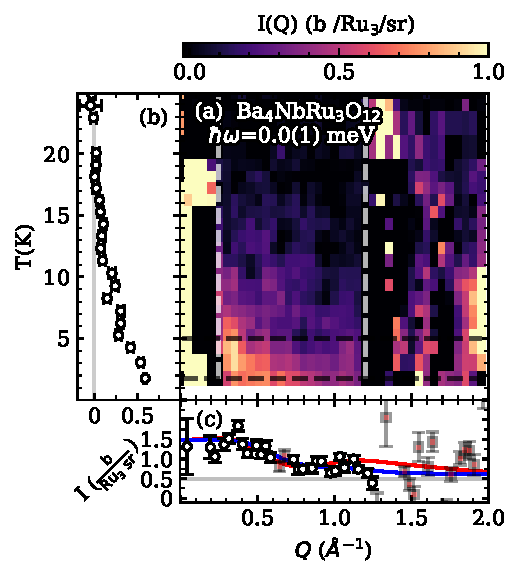
\includegraphics[width=1.0\columnwidth]{Figures/macs_elastic_bnro_compsite.pdf}
    \caption{(a) Temperature dependence of elastic magnetic scattering of Ba$_4$NbRu$_3$O$_{12}$ acquired on the MACS instrument with E$_i$=3.7meV. Averaged signals from temperatures ranging from 20 K to 25 K were subtracted as a background to isolate magnetic signal associated with spin freezing. The energy transfer range contributing to this signal is defined by the elastic resolution of MACS in this configuration which is $\Delta E=0.2$ meV full width at half maximum. (b) Temperature dependence of bulk of magnetic signal integrated within the range of the white lines. The signal dramatically increases below temperatures of 10.0(1) K. (c) Cut along $Q$ integrated in the temperature range shown by the black lines. The red line is a fit described later in the text assuming scattering from Ru ions. The blue line is the same fit but using assuming scattering from a trimer molecular magnet. The red boxes denote points that are contaminated by Bragg peaks and were not used in the fit.}
    \label{el_fig}
\end{figure}


\begin{figure}
    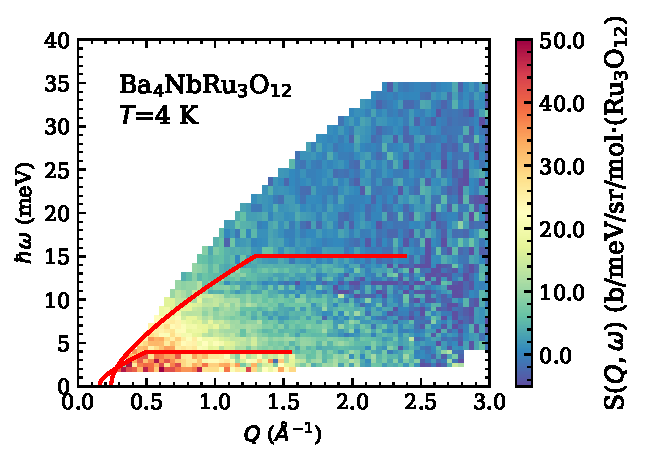
\includegraphics[width=1.0\columnwidth]{Figures/BNRO_magscatter.pdf}
    \caption{Magnetic inelastic neutron scattering spectra of Ba$_4$NbRu$_3$O$_{12}$ measured using the SEQUOIA instrument. High temperature and empty can measurements were used to isolate the magnetic signal as described in the supplementary information. Low temperature measurements were acquired at $T=$4.0(1)  K, with $E_i$=10.5 meV, 25.0 meV, and 50.0 meV. The boundaries between the different $E_i$ configurations are shown by the red dotted lines. The scattering is assosciated with dynamic spin correlations. }
    \label{inel_fig}
\end{figure}

The intensity data from the MACS measurement has been normalized to the integrated intensity of the (10$\bar{1}$) Bragg peak to obtain an absolute measure of the partial differential scattering cross section. For the SEQUIOA measurement, all observable Bragg peaks were used for a similar normalization. An empty aluminum sample can was measured at SEQUOIA to account for the scattering from the sample environment and the sample container. By combining data acquired with the three different values of $E_i$ previously mentioned, we obtained a full spectrum of scattering extending from  $\hbar\omega$=1.5(2) meV to 45 meV energy transfer. An angle and energy dependent absorption correction was applied based on the tabulated absorption cross sections.\cite{sears1992neutron}, but for all measurements absorption is very low ($|T|>96\%$ in all configurations). High temperature measurements were conducted to isolate magnetic scattering from one-phonon scattering. Multiphonon contributions to the scattering were determine using the OCLIMAX software package \cite{Cheng2019SimulationOCLIMAX} and subtracted from the data. Multiple scattering contributions were removed by a model involving a strong incoherent elastic process paired with a weaker coherent inelastic (i.e. phonon) process in conjunction with the OCLIMAX calculations. Further details about these corrections are in Appendix \ref{sec:magiso_appendix}. 

\subsection{Results}
\subsubsection{Elastic Scattering and static correlations}
Temperature dependent magnetic elastic scattering ($|\hbar\omega|<$ 0.2 meV) is shown in Fig \ref{el_fig}. To isolate the elastic magnetic scattering we have subtracted the elastic signal measured for $T=25.0(1)$~K. Upon cooling below $T=15$~K, elastic magnetic scattering appears with the intensity growing precipitously near the $T=8$~K maximum in the specific heat capacity of the material. By integrating over the scattering in Fig. \ref{el_fig}(c), a root mean square (RMS)  moment of $\mu_{static}=1.2(3)\ \mu_B$ is deduced that is static on the time scale of 30 ps associated with the 0.15 meV FWHM energy resolution of the instrument. Though $T<<\Theta_{CW}=155$~K, the elastic scattering does not take the form of Bragg peaks. This signifies that no long range two-point spin correlations develop despite the high density of $S$=1/2 degrees of freedom in this crystalline solid \cite{Nguyen2018GeometricallyInsulator}. Other cases appear in the literature of 2D frustrated magnets with correspondence in temperature dependent elastic magnetic neutron scattering and broad specific heat maxima including NiGa$_2$S$_4$\cite{Nakatsuji2005Physics:Lattice} and SrCr$_{9p}$Ga$_{12-9p}$O$_{19}$\cite{Lee1996Spin-glassMagnet}. The solid lines through the data are theoretical fits to be described in greater detail later, that involve correlations only to nearest molecular neighbors.

\subsubsection{Inelastic Scattering and dynamic correlations}
Fig.~\ref{inel_fig} presents the dynamic spin correlation function ${\cal S}(Q,\omega)$ at $T=4.0$~K obtained by combining background subtracted inelastic neutrons scattering data acquired with three different incident neutron energies. Our study of the elastic scattering already showed there are no magnetic Bragg peaks and therefore we cannot expect any sharp features in the momentum dependence of the data. Instead ${\cal S}(Q,\omega)$ is peaked at low $Q$ and $\hbar\omega$ decreasing with energy transfer on a scale that resembles the Curie-Weiss temperature. This is consistent with dynamic correlations of a macroscopic interacting spin system and clearly contrasts with expectations for intra-molecular excitations, which have a discrete spectrum. 

For a closer examination of the $Q$ and $\hbar\omega$ dependence of these data it is expedient to make the assumption that the dynamical correlation function ${\cal S}(Q,\omega)$ can be approximated as an independent function of $Q$ and $\omega$, i.e.
\begin{eqnarray}
    I(Q,\omega)&=&2r_0^2|\frac{g}{2}F(Q)|^2{\cal S}(Q,\omega) \nonumber \\
    &=&2r_0^2|\frac{g}{2}F(Q)|^2{\cal S}(Q)G(\omega).
    \label{factorization_eq_appendix}
\end{eqnarray}
Within the kinematically accessible range, this is consistent with our data and has been found to be good approximation for a number of frustrated magnetic materials such as for example SrCr$_9$Ga$_{12}$O$_{19}$ \cite{Lee1996Spin-glassMagnet,Yang2015SpinMagnet} where no long ranged correlations develop and no dispersion is apparent in the pattern of scattering. Here we define the spectral function to be unity normalized
\begin{equation}
    \int G(\omega)d\omega =1
    \label{norm_condition}
\end{equation}
while the integral over ${\cal S}(Q)$ yields the effective moment through the total moment sum-rule: 
\begin{equation}
    \mu_{dynamic}^2=3g^2\frac{\int Q^2 {\cal S}(Q)dQ}{\int Q^2 dQ}.
    \label{total_moment_eq}
\end{equation}
The assumption allows for the determination of ${\cal S}(Q)$ and $G(\omega)$ using all the data despite the skewed nature of the kinematic constraints.
A fitting protocol was used to project the ${\cal O}(N_Q\times N_\omega )$ experimental pixels onto $N_Q$ values of  $|F(Q)|^2{\cal S}(Q)$ and $N_\omega$ values of the local excitation spectrum $G(\omega )$ throughout the  factorized range of Q and $\omega$.  

\begin{figure}
    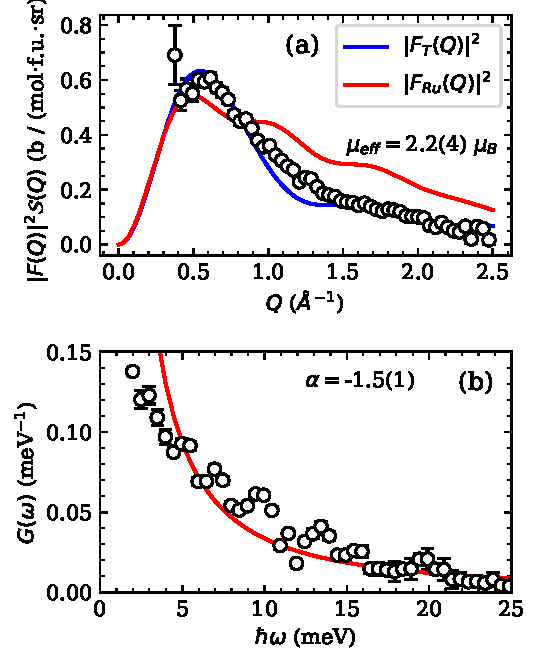
\includegraphics[width=1.0\columnwidth]{Figures/bnro_factorizations.pdf}
    \caption{G($\omega$) spectral weight extracted from least squares fitting of the magnetic neutron spectrum of Ba$_4$NbRu$_3$O$_{12}$. The diffuse inelastic scattering phenomonologically fits to a power law of the exponent $\rho$ shown as the red line. The mean spectral weight is found to be at 10.1meV. }
    \label{fig:factorizations}
\end{figure}

The local ($Q-$ averaged) spectrum inferred from this analysis (Fig. \ref{fig:factorizations}(b)) is continuous and devoid of resonances up to 15 meV, which matches the Curie-Weiss energy scale. This diffuse part of the spectrum can be well described by a phenomenological power law of the form $(\hbar\omega)^{\alpha}$ with an exponent of $\alpha =1.5(1)$ as shown by the red line in Fig. \ref{fig:factorizations}. Any finite sized spin cluster has a discrete excitation spectrum that produces sharp peaks in the low $T$ spectrum of neutron scattering. In Ba$_4$NbRu$_3$O$_{12}$, transport and diffraction data points to an insulating crystalline solid, which barring an undetected static electronic disorder, cannot produce a continuum of scattering, which is not consistent with these data and indicates a wide distribution of clustering length scales. These data are thus is an important indication that the quantum magnetism of Ba$_4$NbRu$_3$O$_{12}$ is collective on the energy scale set by $\Theta_{CW}$. 

The dynamic spatial correlations are reflected by $|F(Q)|^2{\cal S}(Q)$ displayed in Fig.~\ref{fig:factorizations}(a). The function clearly decreases with $Q$, which is consistent with a magnetic signal limited by the atomic form factor $|F(Q)|^2$. in addition, the data display oscillations that are not present in the Ru$^{4+}$  form factor  and that must be ascribed to inter-site spin correlations.

Applying Eq.~\ref{total_moment_eq} and the nominal formfactor for Ru$^{4+}$ we obtain an effective RMS fluctuating moment of $\mu_{dynamic}=2.2(6)\ \mu_B$ which may be compared with the RMS static moment of $\mu_{static}=1.2(3)~\mu_B$ inferred from the elastic scattering. The total effective moment obtained from the scattering data is $\mu_{eff}=\sqrt{\mu_{static}^2+\mu_{dynamic}^2}=2.5(7)~\mu_B$, which is consistent with the effective moment of 2.59$~\mu_B$ inferred from high $T$ susceptibility data. This provides an important check on the background subtraction and normalization procedures employed. 

For a fully ordered spin$-S$ magnet the ratio of mean squared dynamic to mean squared static moment is $(S(S+1)-S^2)/S^2=1/S$ corresponding to a value of $1/S=2$ for spin-1/2. The larger number of $\mu_{dynamic}^2/\mu_{static}^2=3(1)$ that we obtain for Ba$_4$NbRu$_3$O$_{12}$ is a suggestive indication that we are not dealing with a conventional Néel like product state of fully frozen spins. Conversely, ratio falls far short of expectations for a quantum spin liquid where  $\mu_{static}^2=0$.  

\section{Analysis and Discussion}

\subsubsection{Correlation Functions}

The factorized form for ${\cal S}(Q,\omega)$ implies the following form for the dynamic component of the equal time correlation function:
\begin{eqnarray}
{\cal S}(Q)&=& \frac{1}{\langle \hbar\omega\rangle}\int {\cal S}(Q,\omega)\omega d\omega \label{fmfac}\\ 
&=&-\sum_{\textbf{d}} \frac{J_\textbf{d}
\langle \textbf{S}_\textbf{r}\cdot\textbf{S}_{\textbf{r}+\textbf{d}}\rangle}{3\langle \hbar\omega\rangle} \Big[1 - \frac{\sin(Qd)}{Qd}\Big]
\label{first_moment_eq}
\end{eqnarray}
Here $\{ \textbf{d}\}$ denotes the set of all displacement vectors between spins that interact with each other. Eq~\ref{factorization_eq_appendix} was used to obtain Eq.~\ref{fmfac} with the definition $\langle \hbar\omega\rangle=\int g(\omega) \omega d\omega$.  Considering only Heisenberg-like interactions between Ru$_3$O$_{12}$ sites, the first moment sum rule is used to obtain Eq.~\ref{first_moment_eq} \cite{Hohenberg1974,zaliznyak2005magnetic}. The equation implies that the correlation length associated with a factorized dynamic correlation function is capped at the largest spacing between interacting spins $\xi={\rm max}({\textbf{d}})$. The Heisenberg spin Hamiltonian as follows: 
\begin{equation}
    {\cal H}=\frac{1}{2}\sum_{\textbf{r},\textbf{d}} J_\textbf{d} \textbf{S}_\textbf{r}\cdot \textbf{S}_{\textbf{r}+\textbf{d}}.
    \label{eq:hamiltonian}
\end{equation}
Here  $\{ \textbf{r}\}$ are position vectors for all spins and since each interacting spin pair appears twice in this summation the factor $1/2$ ensures that $J_\textbf{d}$ is the exchange energy for spin pair $\textbf{d}$. 

Equation~\ref{first_moment_eq} allows the extraction of the product of bond energies and two-spin correlations, $J_\textbf{d}
\langle \textbf{S}_\textbf{r}\cdot\textbf{S}_{\textbf{r}+\textbf{d}}\rangle$ from a fit to normalized data for ${\cal S}(Q)$ and the value of $\langle\hbar\omega\rangle=10.1$ meV obtained from $G(\omega)$ (Fig.~\ref{ge_fig}). 

The red line in Fig. \ref{fig:factorizations}(a) represents a fit to Eq. \ref{first_moment_eq} assuming nearest and next-nearest neighbor interactions between spins on the triangular lattice. The blue line in the same figure is the same fit but considering the spatial anisotropy of the Ru$_3$O$_{12}$ trimer which is manfested in the magnetif form factor $|F_{Ru,T}(\bm{Q})|^2$. Here the subscripts $Ru$ and $T$ refer to the free-ion Ru$^{4+}$ and the analytical form for the molecular Ru$_3$O$_{12}$ form factor respectively. The corresponding low $T$ excitation spectrum $G(\omega)$ is gapless to within the 1.5 meV energy resolution and extends to 20~meV energy transfer, decreasing monotonically with $\hbar\omega$. 

For the elastic scattering, the description is slightly different. The measured intensity is given by 
\begin{equation}
    I(Q) = 2r_0^2|\frac{g}{2} F(Q)|^2 S_{el}(Q)
    \label{eq:intensity_elastic}
\end{equation}
where $S_{el}(Q)$ is equal time spin correlation function. We directly measure the infinite time spin correlation function $\langle \textbf{S}_i (0)\cdot \textbf{S}_j(\infty)\rangle$ which in the case of diffuse scattering has the following Q-dependence:

\begin{equation}
    S_{el}(Q)=\frac{1}{3}\sum_d^{0,d_1,...}\bigg\{\langle \textbf{S}_o(\infty)\cdot \textbf{S}_d \rangle \frac{\sin(Qd)}{Qd}\bigg\}
\end{equation}
where the allowed interaction vectors $\textbf{d}$ includes the self-correlation term. Written explicitly in terms of intensity this is
\begin{equation}
    I(Q) = \frac{2|\frac{g}{2}F(Q)|^2r_o^2}{3}\sum_d \langle \textbf{S}_o(\infty)\cdot \textbf{S}_d \rangle \frac{\sin(Qd)}{Qd}.
    \label{eq:qfit_elastic}
\end{equation}
The total moment sum rule is also modified slightly, being 
\begin{equation}
    \mu_{static}^2 =3 \frac{\int S_{el}(Q)dQ}{\int Q^2 dQ}.
    \label{eq:sum_rule_elastic}
\end{equation}
The results of fitting the elastic scattering to Eq. \ref{eq:qfit_elastic}(c) when considering trimer magnetic form factor are shown by the blue line in Fig. \ref{el_fig}(c) and the fit parameters are shown in Table \ref{table:fit_params_inelastic}.


\subsection{Comparisons of Elastic and Inelastic Magnetic Scattering}

From the results one can immediately compare the total moments extracted from the elastic and inelastic scattering. This reveals that in the low temperature limit, the majority of spins are fluctuating and that a smaller quantity are frozen at a ratio of $\mu_{dynamic}^2 / \mu_{static}^2 \approx$3:1. Together these represent a total measured magnetic moment of 2.5(7) $\mu_B$ which matches the moment of $2.6\mu_{B}$ extracted from Curie-Weiss expansion of the high temperature magnetization, confirming that all of the magnetic moment in Ba$_4$NbRu$_3$O$_{12}$ is captured in the neutron scattering measurements. Both measurements show a spectrum that is diffuse in Q, with a low momentum transfer peak followed by a smooth decline in intensity. 

Correlation lengths assosciated with each of the spin sites can be extracted from the powder spectra. To do this we apply the functional form given by Eq. \ref{first_moment_eq} allowing for only nearest neighbor ($d_{NN}=5.75\ \AA$) and next-nearest neighbor ($d_{NNN}=9.95\ \AA$) interactions. The result is an acceptable fit to the inelastic measurement shown in Fig. \ref{fq_fig}, and further terms were not found to increase the quality of the fit. The molecular picture clearly is superior in recovering the main features of the scattering, specifically the maxima at low $Q$ that cannot be accounted for in the Ru$^{4+}$ model. The elastic scattering fits well to the form given by Eq. \ref{eq:intensity_elastic} as shown in Fig \ref{el_fig}(c) in both the trimer and free-ion cases. The extracted bond energies $J_d\langle \textbf{S}_o(0) \cdot \textbf{S}_d\rangle$ for the inelastic scattering and relative magnitudes of the spin-spin correlation function $\langle \textbf{S}_o(\infty)\cdot \textbf{S}_d \rangle$ for the elastic scattering are given in Table \ref{table:fit_params_inelastic}. 

The initial evaluation of these moments assumed a magnetic form factor which is equal to that of the free ion Ru$^{4+}$ form factor. Because of the anisotropic geometry of the trimer, the magnetic form factor $|F_T(\textbf{Q})|^2$ originating from the molecular orbital contains significant $Q_z$ dependence ($\hat{z}$ being the Cartesian scattering direction along the c-axis). When evaluated, it can be shown that the scattering in the direction of the nearest neighbor with a non-zero $Q_z$ component is described by a large peak centered at $Q=0.25 \AA^{-1}$ which completely falls off by $Q=1.0 \AA^{-1}$. The details of this evaluation are shown in Appendix B,, but essentially is derived by assuming that the spin density of the trimer may be approximated by three Ru$^{4+}$ ions stacked along the c-axis with the appropriate displacement vector. Using the modified $Q_z$ dependent trimer form factor $|F_T(\textbf{Q})|^2$ rather than the free ion $|F_{Ru}(Q)|^2$, the inelastic spectrum can still be fit well using Eq. \ref{first_moment_eq}.

This method is also applied to the elastic scattering, shown by the blue line in Fig. \ref{el_fig}(c). In this case the molecular form factor only slightly improves the fit, but both the trimer and single-ion treatments can describe the scattering. Single crystal neutron measurements would be able to take better advantage of this anisotropy and would unambiguously determine the nature if the spin degree of freedom in the Ba$_4$NbRu$_3$O$_{12}$ is truly a molecular orbital or of a single-ion nature. 

If it is assumed that the zero and infinite time spin correlators are related by a simple scaling relationship based on the observed magnetic moments
\begin{equation}
\langle \textbf{S}_0(\infty)\cdot\textbf{S}_d\rangle \approx \frac{\mu_{static}^2}{\mu_{dynamic}^2} \langle
\textbf{S}_o(0)\cdot\textbf{S}_d\rangle,
\label{eq:moment_scale}
\end{equation}
one can extract discrete values for $J_d$ which are shown in Table \ref{table:fit_params_inelastic}. In the case of the trimer treatment using $|F_{T}(Q)|^2$, the model is superior in fitting $S(Q)$ as shown in Fig. \ref{fig:factorizations}(a). Only the nearest neighbor term is non-zero beyond error, and considering only this we find $\sum_d J^{T}_d = -0.7(1)$ meV. The results using $|F_{Ru}(Q)|^2$ and only NN and NNN interactions are more poorly constrained, where we find $\sum_d J^{Ru}_d = -1.2(7)$ meV. This is can be compared to what one would expect from the Weiss temperature, $\theta_{CW} = \mu_{eff}^2 / (3k_Bg^2)\sum_d J_d$. For $\theta_{CW}$ = -155~K, $g=2$, and $\mu_{eff}=2.59~\mu_B$ from susceptibility measurements we expect $\sum_d J_d=-1.8$ meV per bond after considering the sixfold nearest and next-nearest neighbor symmetry of the triangular lattice. The extracted values for $J_d$ can only be interpreted as an estimate, but their consistency with what is expected from $\theta_{CW}$ suggests that they are physically reasonable. Even if the absolute magnitudes of the exchange parameters are not precise, we may still consider the signs and relative magnitudes of the interactions. This would mean that the magnetism in Ba$_4$NbRu$_3$O$_{12}$ can be described by a strong antiferromagnetic nearest neighbor exchange on the triangular lattice, followed by a weaker antiferromagnetic exchange with the next nearest neighbor site.  
\begin{center}
\begin{table}
\centering
\noindent 
\begin{tabular}{||c|c|c|c||}
\hline
    Inelastic & d($\angstrom$) & $|F_{Ru}(Q)|^2$ & $|F_{T}(Q)|^2$  \\
    \hline 
     $J_1\langle \textbf{S}_o(0)\cdot \textbf{S}_\textbf{d} \rangle$ (meV)& 5.75 & -0.9(4) & -3.3(2) \\
     $J_2\langle \textbf{S}_o(0)\cdot \textbf{S}_\textbf{d} \rangle$ (meV)& 9.95 & -1.1(4) & -0.2(3) \\
     $J_1$ (meV) & 5.75 & -0.3(1) & -0.7(1)\\
     $J_2$ (meV) & 9.95 & 0.6(7) & 0.0(1)\\
    \hline \hline
    Elastic & d($\angstrom$) & $|F_{Ru}(Q)|^2$ & $|F_{T}(Q)|^2$ \\
    \hline 
     $\langle \textbf{S}_0(\infty) \cdot \textbf{S}_0 \rangle$ & 0 &  0.77(7) & 1.5(1)  \\
     $\langle \textbf{S}_0(\infty) \cdot \textbf{S}_{NN}\rangle$ & 5.75 &  1.1(3) & 0.3(2)  \\
     $\langle \textbf{S}_0(\infty) \cdot \textbf{S}_{NNN}\rangle$& 9.95 &  -0.6(6) &  -0.8(3) \\
     \hline 
\end{tabular}
\caption{Fitting parameters for fits to the inelastic and elastic spectra using Eq. \ref{first_moment_eq} and Eq. \ref{eq:intensity_elastic} . Uncertainties are based on change in fit quality with the variation of each parameter. The interactions are the nearest-neighbor and next-nearest neighbor in the plane of the triangular lattice, and an additional nearest neighbor interlayer interaction. The columns $|F_{Ru}(Q)|^2$ and $|F_{T}(Q)|^2$ denote the results of assuming the Ru$^{4+}$ magnetic form factor $|F_{Ru}(Q)|^2$ and the trimer form factor $|F_{T}(Q)|^2$ respectively. }
\label{table:fit_params_inelastic}
\end{table}
\end{center}

\subsection{Discussion of Energy Spectra and Magnetic Ground State}



The diffuse power law spectra is featureless, and reflects the disordered nature of the magnetism. We have already shown that the present interactions can be described as Heisenberg like, and that a large portion of the spin degrees of freedom remain fluctuating below the freezing temperature. These pictures are not consistent- it is known that NN Heisenberg antiferromagnets have an ordered ground state \cite{Capriotti1999Long-rangeModel,White2007NeelModels}, which is not observed in this case. For Heisenberg spins on a triangular lattice interactions longer than nearest neighbor must be present to suppress the formation of long range order as has been studied extensively through theory\cite{Zhu2015SpinLattice,Iqbal2016SpinAntiferromagnet}. Further, spin freezing should not be possible for Heisenberg spins on a triangular lattice without the introduction of interlayer interactions. These should be visible through the anisotropy molecular form factor $|F_{T}(Q)|^2$. Though our measurements do not have the fidelity to consistently refine interlayer interactions, should single crystalline samples appear we expect that one would become apparent in neutron scattering measurements. Our results then characterize Ba$_4$NbRu$_3$O$_{12}$ as a frustrated molecular magnet with nearest and next nearest neighbor interactions on a triangular lattice, with some interlayer exchange of unclear magnitude driving some of the spins into a frozen state. 

The nature of the remaining spin fluctuations at low temperatures are not clear from this measurement, but they are consistent with at least two possibilities. The first is a spin-liquid like ground state with some portion of the spins being frozen at low temperatures. The second is a partially frozen valence bond solid, in which the fluctuating spins form into distinct singlets across the lattice rather than in a superposition of singlets as in a spin-liquid. Previous calculations of the dynamical spin structure factor for the valence bond solid on the triangular lattice in the context of the spin-liquid candidate compound Herbertsmithite reveal a broad continuum of scattering which is qualitatively similar to our extracted $F(\omega)$ \cite{Shimokawa2015StaticLattices}. This continuum is a result of the excitations of singlets of a variety of length scales, producing spectra that would be similar to our observations. A possible way to distinguish between the two is through the use of extremely high field measurements of magnetization as was recently done for the related compound Ba$_5$CuIr$_3$O$_{12}$ \cite{Volkov2020RandomCrystals}.

\section{Conclusion}

In this work, inelastic neutron scattering has been used to characterize the nature of the low temperature magnetism in Ba$_4$NbRu$_3$O$_{12}$. The unique triangular lattice of J$_{eff}$=1/2 magnetic Ru$_3$O$_{12}$ trimers exhibits no long-range order with approximately one third of the spins freezing at around T=4.0(1) K. A variety of methods have been use to perform a detailed quantitative analysis of both the elastic and inelastic measurements, which reveal a largely featureless spectra that falls off with the magnetic form factor of Ru$^{4+}$. 

The Q-dependence of inelastic scattering is well described by an expansion of a first-moment sum rule assuming Heisenberg interactions, while the elastic scattering is described by real space spin correlations. Both measurements imply the existence of both nearest and next-nearest neighbor interactions. A total moment sum rule confirms that the combined scattering accounts for all of the expected magnetic moment in the sample. The energy dependence of the spectrum shows two distinct excitations which are resolution-limited, which may be excitations within the trimer. The application of a form for the magnetic form factor which takes advantage of the anisotropic geometry of the trimer is also compatible with the scattering which suggests that the molecular magnet description of the Ru$_3$O$_{12}$ trimer may be valid, though the case of single ion physics cannot be ruled out.

The data overall supports a description of a highly frustrated system with possible quasiparticle excitations and avenues for future study. Recently, the related compound Ba$_4$NbIr$_3$O$_{12}$ has been studied and has no freezing transition, leaving the possibility open for a quantum spin-liquid ground state \cite{Nguyen2019Trimer-basedBa4NbIr3O12}. Another very similar quasi-1D material Ba$_5$CuIr$_3$O$_{12}$ has also been studied and is suggested to host a random singlet ground  state \cite{Volkov2020RandomCrystals}. Further, without single crystal samples the exact interactions in Ba$_4$NbRu$_3$O$_{12}$ remain unclear. Spectroscopic studies of single crystal samples are required to answer these remaining queries of the anisotropy of the interactions and the nature of the molecular orbital nature of the material. This may be possible given the recent synthesis of single crystals of the related material Ba$_4$NbIr$_3$O$_{12}$ \cite{Thakur2020CrystalMaterial}, and is the clear direction for future studies. 

\begin{acknowledgements}

This work was supported as part of the Institute for Quantum Matter, an Energy Frontier Research Center funded by the U.S. Department of Energy, Office of Science, Basic Energy Sciences under Award No. DE-SC0019331. Access to MACS was provided by the Center for High Resolution Neutron Scattering, a partnership between the National Institute of Standards and Technology and the National Science Foundation under Agreement No. DMR-1508249. The research at Oak Ridge National Lab's Spallation Neutron Source was sponsored by the U.S. Department of Energy, Office of Basic Energy Sciences.

\end{acknowledgements}

\appendix

\section{Normalization to Bragg Peaks}

We use the Bragg peak intensities to normalize our neutron scattering spectra to absolute units. In general, the measured intensity of an arbitrary Bragg peak is given by 
\begin{equation}
    I(Q,\omega) = A \frac{d^2\sigma}{d\Omega d\omega}.
\end{equation}
where $A$ is the normalization factor. Evaluation of a the cross section from coherent nuclear scattering (a Bragg peak) and solving for the normalization condition gives
\begin{equation}
    A=N\frac{4\pi \int I_{meas}(Q,\omega)Q^2 dQd\omega}{M|F_{HKL}|^2\frac{(2\pi)^3}{V_0}}.
    \label{NC_eq}
\end{equation}
The integral represents the measured Bragg peak intensity, $|F_{HKL}|^2$ is the nuclear structure factor, $M$ is the multiplicity of the Bragg peak, and $V_0$ is the unit cell volume. 

There are a number of factors that introduce error into this method. One is the quantity of sample exposed to the beam and the potential for variations in the neutron flux across the extent of the sample size. Other sources of error include ill-defined instrumental resolution effects, variations in structure factor due to disorder, and multiple peaks will often overlap. Because of these factors, this type of normalization is accompanied by a $\sim$20-30\% error \cite{Xu2013AbsoluteData}. 

\section{Analytic Form for Trimer Form-Factor}

In general, the magnetic form factor of any magnetic scattering goes as the fourier transform of the real space spin distribution, which is often the valence electron wave function. In this text it is referenced as $F(Q)$ and is formally defined as 

\begin{equation}
    F(\textbf{Q})=\int e^{iq\textbf{r}}\rho(\textbf{r})dr.
    \label{ft_eq}
\end{equation}

While this can be evaluated numerically, a simple analytical approach is taken here. In this expression, $\rho(\textbf{r})=|\phi(\textbf{r})|^2$ where $\phi(\textbf{r})$ is the electron wavefunction. In Ba$_4$NbRu$_3$O$_{12}$, there exist two Ru$^{4+}$ ions and one Ru$^{3+}$ ions that combine to form the theorized J$_{eff}$=1/2 trimer magnetic unit. A rough assumption is made to ignore the phase of the wavefunction and assume that these ions have identical magnetic form factors. If this is the case, then the wavefunction of the trimer's valence electron can be evaluated. 
Fig \ref{fig:ff_calc_fig} shows calculated values of $|F(\textbf{Q})|^2$ for the scattering directions in plane, out of plane, and nearest neighbors between the a-b plane. The out of plane form factors are clearly very different from the q-dependence of our observed spectra, which exactly follows the free ion Ru$^{4+}$ form factor.
\begin{figure}
    \centering
    \includegraphics[width=1.0\columnwidth]{Figures/bnro_ffanalyitic.pdf}
    \vspace{-1cm}
    \caption{(a) Calculated anisotropic magnetic form factor of Ba$_4$NbRu$_3$O$_{12}$. The blue line represents in-plane scattering which is identical to the free-ion Ru$^{4+}$ case, the red line is the form factor along the direction of the nearest neighbor interlayer interaction. These neighbors are not directly stacked along the c-axis but instead a bit offset. (b) Powder averaged cross sections (Eq. \ref{powderxc_eq_tot_inel}) for NN and NNN interactions on the a-b plane are shown by the blue lines, and the NN interlayer scattering is shown in red.}
    \label{fig:ff_calc_fig}
\end{figure}

\begin{equation}
    \phi(\textbf{r}) \approx \frac{1}{\sqrt{3}}[ \phi(\textbf{r})+\phi(\textbf{r}-\textbf{d}_o)+\phi(\textbf{r}+\textbf{d}_o)].
    \label{wavefunc_eq}
\end{equation}

Here $\textbf{d}_o$ is the displacement vector between Ru ions within the Ru$_3$O$_{12}$ trimer. Given that this is simply a constant along the c-axis, the form factor is evaluated as
\begin{align}
    |F_T(\textbf{Q})| & = \int e^{i\textbf{q}\cdot\textbf{r}}\frac{1}{3}|\phi(\textbf{r})^2+\phi(\textbf{r})\phi(\textbf{r}-\textbf{d}_o)+\\ \nonumber
                &\phi(\textbf{r})\phi(\textbf{r}+\textbf{d}_o)+\phi(\textbf{r}-\textbf{d}_o)\phi(\textbf{r}+\textbf{d}_o) +\\ \nonumber
                &\phi(\textbf{r}-\textbf{d}_o)^2+\phi(\textbf{r}+\textbf{d}_o)^2|d\textbf{r} \nonumber
\end{align}
where $F_T(\textbf{Q})$ denotes the trimer magnetic form factor. We now make the assumption of no direct orbital overlap between the ruthenium ions, meaning that the cross terms evaluate to zero. This is of course a major simplification and more detailed studies of this system would require a more careful analysis. This would perhaps be done by evaluating the form factor numerically through DFT studies. The form factor is now the following:
\begin{equation}
    |F_{T}(\textbf{Q})| = \int e^{i\textbf{q}\cdot\textbf{r}} \frac{1}{3}( |\phi(\textbf{r})|^2+|\phi(\textbf{r}-\textbf{d}_o)|^2+|\phi(\textbf{r}+\textbf{d}_o)|^2)d\textbf{r}.
    \label{wavfunc_ff_eq}
\end{equation}
This form factor is notably dependent on the z-axis component of the scattering. Finally, the free-ion form factor appears and the expression can be simplified to the following:
\begin{align}
    |F_T(\textbf{Q})| & = \frac{1}{3}\bigg[\int e^{i\textbf{Q}\cdot\textbf{r}}|\phi(\textbf{r})|^2dr+\\ \nonumber
                    &\int e^{i\textbf{Q}\cdot(\textbf{r}-\textbf{d}_o)}|\phi(\textbf{r})|^2dr+\int e^{i\textbf{Q}\cdot(\textbf{r}+\textbf{d}_o)}|\phi(\textbf{r})|^2d\textbf{r}\bigg]
\end{align}
\begin{equation}
    |F(\textbf{Q})|^2=\frac{|F_{Ru}(Q)|^2}{9}(1+2\cos(\textbf{Q}\cdot \textbf{d}_o))^2.
\end{equation}
The revised form factor depends solely on the angle between the momentum transfer $\textbf{Q}$ and Ru-Ru displacement vector within the trimer $\textbf{d}$ with distance $d_0=2.54\ \AA$ . In general, the model used in the first moment sum rule fitting assumes that the spherically averaged neutron scattering cross section goes as the following:
\begin{eqnarray}
    \frac{d\sigma^2}{d\Omega d\hbar\omega} =\frac{r_0^2 g^2}{3}\sum_{d,\alpha} J_d^{\alpha\alpha}\langle \textbf{S}_o^{\alpha}(0)\cdot \textbf{S}_d^{\alpha} \rangle \ldots \nonumber \\
    \int \frac{d\Omega}{4\pi}|F(\textbf{Q})|^2(1-\cos(\textbf{Q}\cdot\textbf{d})).
    \label{powderxc_eq}
\end{eqnarray}

Inserting the evaluated form for the magnetic form factor gives the following analytical expression
\begin{multline}
    \frac{d\sigma^2}{d\Omega d\hbar\omega} =\frac{r_0^2 g^2}{3}\frac{|F_{Ru}(Q)|^2}{9}\sum_{d,\alpha} J_d^{\alpha\alpha}\langle \textbf{S}_o^{\alpha}(0)\cdot \textbf{S}_d^{\alpha} \rangle \ldots \\
    \int \frac{d\Omega}{4\pi}(1+2\cos(\textbf{Q}  \cdot \textbf{d}_o))^2(1-\cos(\textbf{Q}\cdot\textbf{d})).
    \label{powderxc_eq_tot_inel}
\end{multline}
The form of this for the elastic scattering which has a slightly different form is the following
\begin{multline}
    \frac{d\sigma^2}{d\Omega d\hbar\omega} =\frac{r_0^2 g^2}{3}\frac{|F_{Ru}(Q)|^2}{9}\sum_{d,\alpha} J_d^{\alpha\alpha}\langle \textbf{S}_o^{\alpha}(0)\cdot \textbf{S}_d^{\alpha} \rangle \ldots \\
    \int \frac{d\Omega}{4\pi}(1+2\cos(\textbf{Q}  \cdot \textbf{d}_o))^2(\cos(\textbf{Q}\cdot\textbf{d})).
    \label{powderxc_eq_tot_el}
\end{multline}

The anisotropy of the form factor depends explicitly the angle between the scattering vector and the a-b plane of the lattice. In the calculation of a powder average, we take the $\hat{z}$ axis to be perpendicular to the plane formed by the magnetic interaction displacement vector $\textbf{d}$ and the Ru-Ru displacement vector $\textbf{d}_o$. The $\hat{x}$ axis is taken to bisect these two vectors, with the angle between the axis and the vectors being $\psi$. Then, the $\textbf{d}$, $\textbf{d}_o$, and $\textbf{Q}$ vectors can be explicitly written in spherical coordinates as
\begin{gather}
    \textbf{d}= (\hat{x} \cos{\psi} + \hat{y} \sin{\psi})d\\
    \textbf{d}_o = (\hat{x} \cos{\psi} - \hat{y} \sin{\psi})d \\
    \textbf{Q}= Q(\hat{x} \cos{\phi}\sin{\theta} + \hat{y}\sin{\phi}\sin{\theta}+\hat{z}\cos{\theta}).
    \label{coordinate_system_def}
\end{gather}

The dot products in the spherical integration in Eq. \ref{powderxc_eq_tot_inel} and Eq. \ref{powderxc_eq_tot_el} may now be simplified to
\begin{gather}
    \textbf{Q}\cdot \textbf{d} = Qd\sin{\theta}\cos{(\phi - \psi)} \\
    \textbf{Q}\cdot\textbf{d}_o = Qd_o \sin{\theta}\cos{(\phi+\psi)} 
    \label{eq:simplified_coords}
\end{gather}

The deviation from the free-ion Ru behaviour is encompassed purely by the angle $\psi$. In this way we can solve the integral in Eq. \ref{powderxc_eq_tot_inel} to get the following analytical form for $S(Q)$

\begin{multline}
    S(Q) = \frac{|F_{Ru}(Q)|^2}{9} \big\{3+2\frac{\sin{(2Qd_o)}}{2Qd_o} +4\frac{\sin{(Qd_o)}}{Qd_o} -\\
    (3\frac{\sin{(Qd)}}{Qd} + \frac{\sin{(Q|2\textbf{d}_o - \textbf{d}|)}}{Q|2\textbf{d}_o-\textbf{d}|} +\frac{\sin{(Q|2\textbf{d}_o + \textbf{d}|)}}{Q|2\textbf{d}_o - \textbf{d}|}\\
    +2\frac{\sin{(Q|\textbf{d}_o - \textbf{d}|)}}{Q|\textbf{d}_o - \textbf{d}|} + 2\frac{\sin{(Q|\textbf{d}_o + \textbf{d}|)}}{Q|\textbf{d}_o - \textbf{d}|})\big\}. 
    \label{eq:exact_sq_long}
\end{multline}

This is simplified when $\textbf{d} \perp \textbf{d}_o$ as in the case of in-plane interactions. Then, the form simplifies to
\begin{multline}
    S(Q) = \frac{|F(Q)|^2}{9}\big\{ 3 + 2 \frac{\sin{(2Qd_o)}}{2Qd_o} + 4 \frac{\sin{(Qd_o)}}{Qd_o}\\
    -(3\frac{\sin{(Qd)}}{Qd} + 2\frac{\sin{(Q\sqrt{4d_o^2 + d^2})}}{Q\sqrt{4d_o^2 +d^2}}\\
    +2\frac{\sin{(Q\sqrt{d_o^2 + d^2})}}{Q\sqrt{d_o^2 + d^2}})\big\}
    \label{eq:exact_sq}
\end{multline}

In this way, we get a good approximation of the anisotropic nature of the scattering from the molecular magnet.

\section{Multiphonon Corrections using OCLIMAX}
\label{sec:magscatter_appendix}
A conventional method of removing phonons from powder neutron scattering measurements is to perform two measurements, one at high temperature and one at low temperature, then assume that the inelastic scattering in the high temperature spectra is dominated by phonon scattering rather than magnetic scattering. This is done in the following way

\begin{equation}
    \bar{I}(Q,\omega) = I_{low}(Q,\omega) - \frac{1-e^{-\beta_H\omega}}{1-e^{-\beta_L\omega}}I_{high}(Q,\omega).
    \label{phonon_sub_eq}
\end{equation}

In simple cases this removes all influence of phonons and the remaining intensity is entirely magnetic. For our data this correction leaves a high-Q background which makes any kind of quantitative analysis difficult. The simple subtraction described here does not properly handle processes like multiple scattering and multiphonon scattering. The cross-sections of these processes can end up involving Q-independent terms, giving spurious intensity at high Q. We approximate the contributions to the measured scattering in the following way

\begin{equation}
\label{eq:bnro_scatter_contribs}
I(Q,\hbar\omega) = I_{mag}(Q,\hbar\omega) + I_{ph}^1(Q,\hbar\omega) + I_{ph}^{n}(Q,\hbar\omega) + I_{m}(Q,\hbar\omega).
\end{equation}

Here, the total observed intensity is a linear combination of the desired magnetic scattering $I_{mag}$, single-event phonon scattering $I_{ph}^1$, multiphonon scattering $I_{ph}^n$, and multiple scattering $I_{m}$. 
To overcome this a DFT simulation of the structure was performed in conjunction with a model of the multiphonon scattering using the OCLIMAX software.



\section{Details of OCLIMAX Calculations}
\label{sec:oclimax}
DFT calculations of Ba$_4$NbRu$_3$O$_{12}$ were performed using the VASP Package\cite{Kresse1996EfficientSet}. The calculation used the Projector Augmented Wave\cite{Blochl1994ProjectorMethod,Kresse1999FromMethod} method to describe the effects of core electrons, and the Perdew-Berke-Ernzerhof\cite{Perdew1996GeneralizedSimple} implementation of the Generalized Gradient Approximation for the exchange-correlation functional. The electronic structure was calculated on a 6x6x1 $\Gamma$-centered mesh. Force constants were calculated using Density Functional Perturbation THeory (DFPT) in VASP, and the vibrational eigen-frequencies and modes were then calculated by solving the dynamical matrix using Phononpy\cite{Togo2015FirstScience}. The OCLIMAX\cite{Cheng2019SimulationOCLIMAX} software was then used to convert the DFT-calculated phonon results to a simulated INS spectra, which includes both the vibrational modes and multiphonon contributions. Multiple scattering effects were not included in this calculation, as it is an exact calculation of $S(Q,\omega)$ for scattering events involving multiple phonons rather than a Monte-Carlo type method. In this way the multiphonon contributions were sufficiently removed, and the remainder of the signal that is not described well by the simulation is dominated by single-phonon processes as in Fig \ref{dftfig}. These contributions can then be removed in the more conventional way as in Eq (\ref{phonon_sub_eq}). 

\begin{figure*}
    \centering
    \includegraphics[width=0.7\textwidth]{Figures/BNRO_multscatter_oclimax.pdf}
    \caption{(a) Normalized direct scattering measured at E$_i$=50 meV, $T$=4 K. (b) Best fit to multiple scattering using OCLIMAX calculations and the form of Eq. \ref{eq:oclimaxmultscatter}. Scattering below the kinematic limit only includes the calculated $Q$-independent multiple scattering. (c) Difference between the first two plots, showing small deviations that are corrected for by Bose-Einstein subtraction. 
    \label{fig:multscatter_bnro}}
\end{figure*}
\bibliography{refs}% Produces the bibliography via BibTeX.

\end{document}
%
% ****** End of file apssamp.tex ******
